%%
%
\documentclass[10pt,journal,compsoc]{IEEEtran}


%%%%%%%%%%%%%%%%%
%CUSTOM COMMANDS%
%%%%%%%%%%%%%%%%%
%Combinatorial notation
%From https://tex.stackexchange.com/questions/107125/is-there-a-command-to-write-the-form-of-a-combination-or-permutation
\newcommand*{\Perm}[2]{{}^{#1}\!P_{#2}}%
\newcommand*{\Comb}[2]{{}^{#1}C_{#2}}%

%For inserting code
\usepackage{listings}
%https://www.sharelatex.com/learn/Code_listing

\usepackage{graphicx}

% Some very useful LaTeX packages include:
% (uncomment the ones you want to load)




% *** MISC UTILITY PACKAGES ***
%
%\usepackage{ifpdf}
% Heiko Oberdiek's ifpdf.sty is very useful if you need conditional
% compilation based on whether the output is pdf or dvi.
% usage:
% \ifpdf
%   % pdf code
% \else
%   % dvi code
% \fi
% The latest version of ifpdf.sty can be obtained from:
% http://www.ctan.org/pkg/ifpdf
% Also, note that IEEEtran.cls V1.7 and later provides a builtin
% \ifCLASSINFOpdf conditional that works the same way.
% When switching from latex to pdflatex and vice-versa, the compiler may
% have to be run twice to clear warning/error messages.






% *** CITATION PACKAGES ***
%
\usepackage[nocompress]{cite}

% cite.sty was written by Donald Arseneau
% V1.6 and later of IEEEtran pre-defines the format of the cite.sty package
% \cite{} output to follow that of the IEEE. Loading the cite package will
% result in citation numbers being automatically sorted and properly
% "compressed/ranged". e.g., [1], [9], [2], [7], [5], [6] without using
% cite.sty will become [1], [2], [5]--[7], [9] using cite.sty. cite.sty's
% \cite will automatically add leading space, if needed. Use cite.sty's
% noadjust option (cite.sty V3.8 and later) if you want to turn this off
% such as if a citation ever needs to be enclosed in parenthesis.
% cite.sty is already installed on most LaTeX systems. Be sure and use
% version 5.0 (2009-03-20) and later if using hyperref.sty.
% The latest version can be obtained at:
% http://www.ctan.org/pkg/cite
% The documentation is contained in the cite.sty file itself.
%
% Note that some packages require special options to format as the Computer
% Society requires. In particular, Computer Society  papers do not use
% compressed citation ranges as is done in typical IEEE papers
% (e.g., [1]-[4]). Instead, they list every citation separately in order
% (e.g., [1], [2], [3], [4]). To get the latter we need to load the cite
% package with the nocompress option which is supported by cite.sty v4.0
% and later.





% *** GRAPHICS RELATED PACKAGES ***
%
\ifCLASSINFOpdf
  % \usepackage[pdftex]{graphicx}
  % declare the path(s) where your graphic files are
  % \graphicspath{{../pdf/}{../jpeg/}}
  % and their extensions so you won't have to specify these with
  % every instance of \includegraphics
  % \DeclareGraphicsExtensions{.pdf,.jpeg,.png}
\else
  % or other class option (dvipsone, dvipdf, if not using dvips). graphicx
  % will default to the driver specified in the system graphics.cfg if no
  % driver is specified.
  % \usepackage[dvips]{graphicx}
  % declare the path(s) where your graphic files are
  % \graphicspath{{../eps/}}
  % and their extensions so you won't have to specify these with
  % every instance of \includegraphics
  % \DeclareGraphicsExtensions{.eps}
\fi
% graphicx was written by David Carlisle and Sebastian Rahtz. It is
% required if you want graphics, photos, etc. graphicx.sty is already
% installed on most LaTeX systems. The latest version and documentation
% can be obtained at: 
% http://www.ctan.org/pkg/graphicx
% Another good source of documentation is "Using Imported Graphics in
% LaTeX2e" by Keith Reckdahl which can be found at:
% http://www.ctan.org/pkg/epslatex
%
% latex, and pdflatex in dvi mode, support graphics in encapsulated
% postscript (.eps) format. pdflatex in pdf mode supports graphics
% in .pdf, .jpeg, .png and .mps (metapost) formats. Users should ensure
% that all non-photo figures use a vector format (.eps, .pdf, .mps) and
% not a bitmapped formats (.jpeg, .png). The IEEE frowns on bitmapped formats
% which can result in "jaggedy"/blurry rendering of lines and letters as
% well as large increases in file sizes.
%
% You can find documentation about the pdfTeX application at:
% http://www.tug.org/applications/pdftex





% *** MATH PACKAGES ***
%
\usepackage{amsmath}
% A popular package from the American Mathematical Society that provides
% many useful and powerful commands for dealing with mathematics.
%
% Note that the amsmath package sets \interdisplaylinepenalty to 10000
% thus preventing page breaks from occurring within multiline equations. Use:
%\interdisplaylinepenalty=2500
% after loading amsmath to restore such page breaks as IEEEtran.cls normally
% does. amsmath.sty is already installed on most LaTeX systems. The latest
% version and documentation can be obtained at:
% http://www.ctan.org/pkg/amsmath





% *** SPECIALIZED LIST PACKAGES ***
%\usepackage{acronym}
% acronym.sty was written by Tobias Oetiker. This package provides tools for
% managing documents with large numbers of acronyms. (You don't *have* to
% use this package - unless you have a lot of acronyms, you may feel that
% such package management of them is bit of an overkill.)
% Do note that the acronym environment (which lists acronyms) will have a
% problem when used under IEEEtran.cls because acronym.sty relies on the
% description list environment - which IEEEtran.cls has customized for
% producing IEEE style lists. A workaround is to declared the longest
% label width via the IEEEtran.cls \IEEEiedlistdecl global control:
%
% \renewcommand{\IEEEiedlistdecl}{\IEEEsetlabelwidth{SONET}}
% \begin{acronym}
%
% \end{acronym}
% \renewcommand{\IEEEiedlistdecl}{\relax}% remember to reset \IEEEiedlistdecl
%
% instead of using the acronym environment's optional argument.
% The latest version and documentation can be obtained at:
% http://www.ctan.org/pkg/acronym


%\usepackage{algorithmic}
% algorithmic.sty was written by Peter Williams and Rogerio Brito.
% This package provides an algorithmic environment fo describing algorithms.
% You can use the algorithmic environment in-text or within a figure
% environment to provide for a floating algorithm. Do NOT use the algorithm
% floating environment provided by algorithm.sty (by the same authors) or
% algorithm2e.sty (by Christophe Fiorio) as the IEEE does not use dedicated
% algorithm float types and packages that provide these will not provide
% correct IEEE style captions. The latest version and documentation of
% algorithmic.sty can be obtained at:
% http://www.ctan.org/pkg/algorithms
% Also of interest may be the (relatively newer and more customizable)
% algorithmicx.sty package by Szasz Janos:
% http://www.ctan.org/pkg/algorithmicx




% *** ALIGNMENT PACKAGES ***
%
%\usepackage{array}
% Frank Mittelbach's and David Carlisle's array.sty patches and improves
% the standard LaTeX2e array and tabular environments to provide better
% appearance and additional user controls. As the default LaTeX2e table
% generation code is lacking to the point of almost being broken with
% respect to the quality of the end results, all users are strongly
% advised to use an enhanced (at the very least that provided by array.sty)
% set of table tools. array.sty is already installed on most systems. The
% latest version and documentation can be obtained at:
% http://www.ctan.org/pkg/array


%\usepackage{mdwmath}
%\usepackage{mdwtab}
% Also highly recommended is Mark Wooding's extremely powerful MDW tools,
% especially mdwmath.sty and mdwtab.sty which are used to format equations
% and tables, respectively. The MDWtools set is already installed on most
% LaTeX systems. The lastest version and documentation is available at:
% http://www.ctan.org/pkg/mdwtools


% IEEEtran contains the IEEEeqnarray family of commands that can be used to
% generate multiline equations as well as matrices, tables, etc., of high
% quality.


%\usepackage{eqparbox}
% Also of notable interest is Scott Pakin's eqparbox package for creating
% (automatically sized) equal width boxes - aka "natural width parboxes".
% Available at:
% http://www.ctan.org/pkg/eqparbox




% *** SUBFIGURE PACKAGES ***
%\ifCLASSOPTIONcompsoc
%  \usepackage[caption=false,font=footnotesize,labelfont=sf,textfont=sf]{subfig}
%\else
%  \usepackage[caption=false,font=footnotesize]{subfig}
%\fi
% subfig.sty, written by Steven Douglas Cochran, is the modern replacement
% for subfigure.sty, the latter of which is no longer maintained and is
% incompatible with some LaTeX packages including fixltx2e. However,
% subfig.sty requires and automatically loads Axel Sommerfeldt's caption.sty
% which will override IEEEtran.cls' handling of captions and this will result
% in non-IEEE style figure/table captions. To prevent this problem, be sure
% and invoke subfig.sty's "caption=false" package option (available since
% subfig.sty version 1.3, 2005/06/28) as this is will preserve IEEEtran.cls
% handling of captions.
% Note that the Computer Society format requires a sans serif font rather
% than the serif font used in traditional IEEE formatting and thus the need
% to invoke different subfig.sty package options depending on whether
% compsoc mode has been enabled.
%
% The latest version and documentation of subfig.sty can be obtained at:
% http://www.ctan.org/pkg/subfig




% *** FLOAT PACKAGES ***
%
%\usepackage{fixltx2e}
% fixltx2e, the successor to the earlier fix2col.sty, was written by
% Frank Mittelbach and David Carlisle. This package corrects a few problems
% in the LaTeX2e kernel, the most notable of which is that in current
% LaTeX2e releases, the ordering of single and double column floats is not
% guaranteed to be preserved. Thus, an unpatched LaTeX2e can allow a
% single column figure to be placed prior to an earlier double column
% figure.
% Be aware that LaTeX2e kernels dated 2015 and later have fixltx2e.sty's
% corrections already built into the system in which case a warning will
% be issued if an attempt is made to load fixltx2e.sty as it is no longer
% needed.
% The latest version and documentation can be found at:
% http://www.ctan.org/pkg/fixltx2e


%\usepackage{stfloats}
% stfloats.sty was written by Sigitas Tolusis. This package gives LaTeX2e
% the ability to do double column floats at the bottom of the page as well
% as the top. (e.g., "\begin{figure*}[!b]" is not normally possible in
% LaTeX2e). It also provides a command:
%\fnbelowfloat
% to enable the placement of footnotes below bottom floats (the standard
% LaTeX2e kernel puts them above bottom floats). This is an invasive package
% which rewrites many portions of the LaTeX2e float routines. It may not work
% with other packages that modify the LaTeX2e float routines. The latest
% version and documentation can be obtained at:
% http://www.ctan.org/pkg/stfloats
% Do not use the stfloats baselinefloat ability as the IEEE does not allow
% \baselineskip to stretch. Authors submitting work to the IEEE should note
% that the IEEE rarely uses double column equations and that authors should try
% to avoid such use. Do not be tempted to use the cuted.sty or midfloat.sty
% packages (also by Sigitas Tolusis) as the IEEE does not format its papers in
% such ways.
% Do not attempt to use stfloats with fixltx2e as they are incompatible.
% Instead, use Morten Hogholm'a dblfloatfix which combines the features
% of both fixltx2e and stfloats:
%
% \usepackage{dblfloatfix}
% The latest version can be found at:
% http://www.ctan.org/pkg/dblfloatfix


%\ifCLASSOPTIONcaptionsoff
%  \usepackage[nomarkers]{endfloat}
% \let\MYoriglatexcaption\caption
% \renewcommand{\caption}[2][\relax]{\MYoriglatexcaption[#2]{#2}}
%\fi
% endfloat.sty was written by James Darrell McCauley, Jeff Goldberg and 
% Axel Sommerfeldt. This package may be useful when used in conjunction with 
% IEEEtran.cls'  captionsoff option. Some IEEE journals/societies require that
% submissions have lists of figures/tables at the end of the paper and that
% figures/tables without any captions are placed on a page by themselves at
% the end of the document. If needed, the draftcls IEEEtran class option or
% \CLASSINPUTbaselinestretch interface can be used to increase the line
% spacing as well. Be sure and use the nomarkers option of endfloat to
% prevent endfloat from "marking" where the figures would have been placed
% in the text. The two hack lines of code above are a slight modification of
% that suggested by in the endfloat docs (section 8.4.1) to ensure that
% the full captions always appear in the list of figures/tables - even if
% the user used the short optional argument of \caption[]{}.
% IEEE papers do not typically make use of \caption[]'s optional argument,
% so this should not be an issue. A similar trick can be used to disable
% captions of packages such as subfig.sty that lack options to turn off
% the subcaptions:
% For subfig.sty:
% \let\MYorigsubfloat\subfloat
% \renewcommand{\subfloat}[2][\relax]{\MYorigsubfloat[]{#2}}
% However, the above trick will not work if both optional arguments of
% the \subfloat command are used. Furthermore, there needs to be a
% description of each subfigure *somewhere* and endfloat does not add
% subfigure captions to its list of figures. Thus, the best approach is to
% avoid the use of subfigure captions (many IEEE journals avoid them anyway)
% and instead reference/explain all the subfigures within the main caption.
% The latest version of endfloat.sty and its documentation can obtained at:
% http://www.ctan.org/pkg/endfloat
%
% The IEEEtran \ifCLASSOPTIONcaptionsoff conditional can also be used
% later in the document, say, to conditionally put the References on a 
% page by themselves.





% *** PDF, URL AND HYPERLINK PACKAGES ***
%
\usepackage{url}
% url.sty was written by Donald Arseneau. It provides better support for
% handling and breaking URLs. url.sty is already installed on most LaTeX
% systems. The latest version and documentation can be obtained at:
% http://www.ctan.org/pkg/url
% Basically, \url{my_url_here}.


% NOTE: PDF thumbnail features are not required in IEEE papers
%       and their use requires extra complexity and work.
%\ifCLASSINFOpdf
%  \usepackage[pdftex]{thumbpdf}
%\else
%  \usepackage[dvips]{thumbpdf}
%\fi
% thumbpdf.sty and its companion Perl utility were written by Heiko Oberdiek.
% It allows the user a way to produce PDF documents that contain fancy
% thumbnail images of each of the pages (which tools like acrobat reader can
% utilize). This is possible even when using dvi->ps->pdf workflow if the
% correct thumbpdf driver options are used. thumbpdf.sty incorporates the
% file containing the PDF thumbnail information (filename.tpm is used with
% dvips, filename.tpt is used with pdftex, where filename is the base name of
% your tex document) into the final ps or pdf output document. An external
% utility, the thumbpdf *Perl script* is needed to make these .tpm or .tpt
% thumbnail files from a .ps or .pdf version of the document (which obviously
% does not yet contain pdf thumbnails). Thus, one does a:
% 
% thumbpdf filename.pdf 
%
% to make a filename.tpt, and:
%
% thumbpdf --mode dvips filename.ps
%
% to make a filename.tpm which will then be loaded into the document by
% thumbpdf.sty the NEXT time the document is compiled (by pdflatex or
% latex->dvips->ps2pdf). Users must be careful to regenerate the .tpt and/or
% .tpm files if the main document changes and then to recompile the
% document to incorporate the revised thumbnails to ensure that thumbnails
% match the actual pages. It is easy to forget to do this!
% 
% Unix systems come with a Perl interpreter. However, MS Windows users
% will usually have to install a Perl interpreter so that the thumbpdf
% script can be run. The Ghostscript PS/PDF interpreter is also required.
% See the thumbpdf docs for details. The latest version and documentation
% can be obtained at.
% http://www.ctan.org/pkg/thumbpdf


% NOTE: PDF hyperlink and bookmark features are not required in IEEE
%       papers and their use requires extra complexity and work.
% *** IF USING HYPERREF BE SURE AND CHANGE THE EXAMPLE PDF ***
% *** TITLE/SUBJECT/AUTHOR/KEYWORDS INFO BELOW!!           ***
\newcommand\MYhyperrefoptions{bookmarks=true,bookmarksnumbered=true,
pdfpagemode={UseOutlines},plainpages=false,pdfpagelabels=true,
colorlinks=true,linkcolor={black},citecolor={black},urlcolor={black},
pdftitle={Bare Demo of IEEEtran.cls for Computer Society Journals},%<!CHANGE!
pdfsubject={Typesetting},%<!CHANGE!
pdfauthor={Michael D. Shell},%<!CHANGE!
pdfkeywords={Computer Society, IEEEtran, journal, LaTeX, paper,
             template}}%<^!CHANGE!
%\ifCLASSINFOpdf
%\usepackage[\MYhyperrefoptions,pdftex]{hyperref}
%\else
%\usepackage[\MYhyperrefoptions,breaklinks=true,dvips]{hyperref}
%\usepackage{breakurl}
%\fi
% One significant drawback of using hyperref under DVI output is that the
% LaTeX compiler cannot break URLs across lines or pages as can be done
% under pdfLaTeX's PDF output via the hyperref pdftex driver. This is
% probably the single most important capability distinction between the
% DVI and PDF output. Perhaps surprisingly, all the other PDF features
% (PDF bookmarks, thumbnails, etc.) can be preserved in
% .tex->.dvi->.ps->.pdf workflow if the respective packages/scripts are
% loaded/invoked with the correct driver options (dvips, etc.). 
% As most IEEE papers use URLs sparingly (mainly in the references), this
% may not be as big an issue as with other publications.
%
% That said, Vilar Camara Neto created his breakurl.sty package which
% permits hyperref to easily break URLs even in dvi mode.
% Note that breakurl, unlike most other packages, must be loaded
% AFTER hyperref. The latest version of breakurl and its documentation can
% be obtained at:
% http://www.ctan.org/pkg/breakurl
% breakurl.sty is not for use under pdflatex pdf mode.
%
% The advanced features offer by hyperref.sty are not required for IEEE
% submission, so users should weigh these features against the added
% complexity of use.
% The package options above demonstrate how to enable PDF bookmarks
% (a type of table of contents viewable in Acrobat Reader) as well as
% PDF document information (title, subject, author and keywords) that is
% viewable in Acrobat reader's Document_Properties menu. PDF document
% information is also used extensively to automate the cataloging of PDF
% documents. The above set of options ensures that hyperlinks will not be
% colored in the text and thus will not be visible in the printed page,
% but will be active on "mouse over". USING COLORS OR OTHER HIGHLIGHTING
% OF HYPERLINKS CAN RESULT IN DOCUMENT REJECTION BY THE IEEE, especially if
% these appear on the "printed" page. IF IN DOUBT, ASK THE RELEVANT
% SUBMISSION EDITOR. You may need to add the option hypertexnames=false if
% you used duplicate equation numbers, etc., but this should not be needed
% in normal IEEE work.
% The latest version of hyperref and its documentation can be obtained at:
% http://www.ctan.org/pkg/hyperref





% *** Do not adjust lengths that control margins, column widths, etc. ***
% *** Do not use packages that alter fonts (such as pslatex).         ***
% There should be no need to do such things with IEEEtran.cls V1.6 and later.
% (Unless specifically asked to do so by the journal or conference you plan
% to submit to, of course. )


% correct bad hyphenation here
\hyphenation{op-tical net-works semi-conduc-tor}


\begin{document}
%
% paper title
% Titles are generally capitalized except for words such as a, an, and, as,
% at, but, by, for, in, nor, of, on, or, the, to and up, which are usually
% not capitalized unless they are the first or last word of the title.
% Linebreaks \\ can be used within to get better formatting as desired.
% Do not put math or special symbols in the title.
\title{Effects of the Development of Quantum Computing on NP Difficulty Problems}
%
%
% author names and IEEE memberships
% note positions of commas and nonbreaking spaces ( ~ ) LaTeX will not break
% a structure at a ~ so this keeps an author's name from being broken across
% two lines.
% use \thanks{} to gain access to the first footnote area
% a separate \thanks must be used for each paragraph as LaTeX2e's \thanks
% was not built to handle multiple paragraphs
%
%
%\IEEEcompsocitemizethanks is a special \thanks that produces the bulleted
% lists the Computer Society journals use for "first footnote" author
% affiliations. Use \IEEEcompsocthanksitem which works much like \item
% for each affiliation group. When not in compsoc mode,
% \IEEEcompsocitemizethanks becomes like \thanks and
% \IEEEcompsocthanksitem becomes a line break with idention. This
% facilitates dual compilation, although admittedly the differences in the
% desired content of \author between the different types of papers makes a
% one-size-fits-all approach a daunting prospect. For instance, compsoc 
% journal papers have the author affiliations above the "Manuscript
% received ..."  text while in non-compsoc journals this is reversed. Sigh.

\author{Matt Fletcher}
% note need leading \protect in front of \\ to get a newline within \thanks as
% \\ is fragile and will error, could use \hfil\break instead.


% note the % following the last \IEEEmembership and also \thanks - 
% these prevent an unwanted space from occurring between the last author name
% and the end of the author line. i.e., if you had this:
% 
% \author{....lastname \thanks{...} \thanks{...} }
%                     ^------------^------------^----Do not want these spaces!
%
% a space would be appended to the last name and could cause every name on that
% line to be shifted left slightly. This is one of those "LaTeX things". For
% instance, "\textbf{A} \textbf{B}" will typeset as "A B" not "AB". To get
% "AB" then you have to do: "\textbf{A}\textbf{B}"
% \thanks is no different in this regard, so shield the last } of each \thanks
% that ends a line with a % and do not let a space in before the next \thanks.
% Spaces after \IEEEmembership other than the last one are OK (and needed) as
% you are supposed to have spaces between the names. For what it is worth,
% this is a minor point as most people would not even notice if the said evil
% space somehow managed to creep in.



% The paper headers
\markboth{Quantum Computing Effects on Encryption}%
{Shell \MakeLowercase{\textit{et al.}}: Bare Advanced Demo of IEEEtran.cls for IEEE Computer Society Journals}
% The only time the second header will appear is for the odd numbered pages
% after the title page when using the twoside option.
% 
% *** Note that you probably will NOT want to include the author's ***
% *** name in the headers of peer review papers.                   ***
% You can use \ifCLASSOPTIONpeerreview for conditional compilation here if
% you desire.



% The publisher's ID mark at the bottom of the page is less important with
% Computer Society journal papers as those publications place the marks
% outside of the main text columns and, therefore, unlike regular IEEE
% journals, the available text space is not reduced by their presence.
% If you want to put a publisher's ID mark on the page you can do it like
% this:
%\IEEEpubid{0000--0000/00\$00.00~\copyright~2015 IEEE}
% or like this to get the Computer Society new two part style.
%\IEEEpubid{\makebox[\columnwidth]{\hfill 0000--0000/00/\$00.00~\copyright~2015 IEEE}%
%\hspace{\columnsep}\makebox[\columnwidth]{Published by the IEEE Computer Society\hfill}}
% Remember, if you use this you must call \IEEEpubidadjcol in the second
% column for its text to clear the IEEEpubid mark (Computer Society journal
% papers don't need this extra clearance.)



% use for special paper notices
%\IEEEspecialpapernotice{(Invited Paper)}



% for Computer Society papers, we must declare the abstract and index terms
% PRIOR to the title within the \IEEEtitleabstractindextext IEEEtran
% command as these need to go into the title area created by \maketitle.
% As a general rule, do not put math, special symbols or citations
% in the abstract or keywords.
\IEEEtitleabstractindextext{%
\begin{abstract}
With general purpose quantum computers on the verge of being invented in the next decade, some worry about what the effects these will have on society. Because quantum computers operate off of rules that break the laws of modern physics, they are far more powerful at computing certain algorithsm. Many secure operations nowadays are only secure due to the extreme difficulty in solving the math problems that they are built from. Two common examples of these operations are RSA Encryption and blockchain. RSA's security lies in prime factorization, and blockchain's security lies in the difficulty of its hashing algorithm.  Since the 1980's, the RSA Encryption algorithm has been used as a near foolproof method of encrypting sensitive data sent over the Internet. Furthermore, blockchain's use in cryptocurrencies is only secure due to the irreversable hashing algorithm used, which ensures the security of the individual accounts. This paper analyzes the effects of quantum computing on the NP applications of RSA Encryption and blockchain, as well as a few other applications in the modern world. 
\end{abstract}

% Note that keywords are not normally used for peerreview papers.
\begin{IEEEkeywords}
Cryptography, Encryption, Quantum computing, P vs NP, Prime Factorization, RSA, Traveling Salesman
\end{IEEEkeywords}}


% make the title area
\maketitle


% To allow for easy dual compilation without having to reenter the
% abstract/keywords data, the \IEEEtitleabstractindextext text will
% not be used in maketitle, but will appear (i.e., to be "transported")
% here as \IEEEdisplaynontitleabstractindextext when compsoc mode
% is not selected <OR> if conference mode is selected - because compsoc
% conference papers position the abstract like regular (non-compsoc)
% papers do!
\IEEEdisplaynontitleabstractindextext
% \IEEEdisplaynontitleabstractindextext has no effect when using
% compsoc under a non-conference mode.


% For peer review papers, you can put extra information on the cover
% page as needed:
% \ifCLASSOPTIONpeerreview
% \begin{center} \bfseries EDICS Category: 3-BBND \end{center}
% \fi
%
% For peerreview papers, this IEEEtran command inserts a page break and
% creates the second title. It will be ignored for other modes.
\IEEEpeerreviewmaketitle


\ifCLASSOPTIONcompsoc
\IEEEraisesectionheading{\section{Introduction}\label{sec:introduction}}
\else
\section{Introduction}
\label{sec:introduction}
\fi
% Computer Society journal (but not conference!) papers do something unusual
% with the very first section heading (almost always called "Introduction").
% They place it ABOVE the main text! IEEEtran.cls does not automatically do
% this for you, but you can achieve this effect with the provided
% \IEEEraisesectionheading{} command. Note the need to keep any \label that
% is to refer to the section immediately after \section in the above as
% \IEEEraisesectionheading puts \section within a raised box.




% The very first letter is a 2 line initial drop letter followed
% by the rest of the first word in caps (small caps for compsoc).
% 
% form to use if the first word consists of a single letter:
% \IEEEPARstart{A}{demo} file is ....
% 
% form to use if you need the single drop letter followed by
% normal text (unknown if ever used by the IEEE):
% \IEEEPARstart{A}{}demo file is ....
% 
% Some journals put the first two words in caps:
% \IEEEPARstart{T}{his demo} file is ....








%%%%%%%%%%%%%%%%%%%%
%BEGINNING OF PAPER%
%%%%%%%%%%%%%%%%%%%%










% Here we have the typical use of a "T" for an initial drop letter
% and "HIS" in caps to complete the first word.
\IEEEPARstart{I}{n 1955, mathematician} John Nash penned a letter to the National Security Agency that would change the face of computing forever\cite{NSA}. 
%https://www.nsa.gov/news-features/declassified-documents/nash-letters/assets/files/nash_letters1.pdf. 
In this letter, he presented a theory about the computational power required to find the solutions to various mathematical problems. In particular, he focused on the art of cryptography, and the length of time necessary to crack an encryption. Up to that point, computer scientists who created algorithms concentrated solely on the required time to solve a particular length of problem. Nash suggested that instead of fixating on the computational duration for a problem with a particular input length, scientists should consider the rate of growth of the problem resolution time given the length of the inputs grew at a linear rate. Furthermore, in lieu of computation time, scientists should focus on the number of computational steps\footnote{A computational step is the number of state changes that the machine processes  in carrying out the set of steps to solve the problem.} required to solve the problem.  The shape of this growth curve would help classify the difficulty of the problem. 

About 3 decades after Nash's letter, a theoretical physicist at MIT named Richard Feynman proposed the idea of a computer that would operate through the use of quantum mechanics. At the time, the idea was simply theoretical, as the technology at the time was not advanced enough to be able to create such a ``quantum computer''. However, scientists began to wonder what the effects of such a computer would have on math and science. This curiosity sparked what has now become the leading edge of innovation in computing power. 


\section{Classifying P and NP Problems}
\IEEEPARstart{T}{he rate} of growth of a problem's difficulty as its input lengths increase can vary drastically. For example, the difficulty of addition of numbers grows at a linear rate. Doubling the number of digits to be added results in approximately double the computation time. Therefore, these problems grow at a linear rate\footnote{Linear growth is still technically considered a polynomial growth of the form $n^k$ with $k=0$.}.  However, problems such as multiplication grow at a slightly faster pace. Doubling the length of the inputs results in a growth of $2^2$ times the number of computational steps. Tripling the length of the input  results in a growth of $3^2$ times the number of computational steps. This growth may be somewhat rapid, but can be expressed as a polynomial\footnote{A polynomial is an expression that can be written in the form $a_{n}x^{n}+a_{n-1}x^{n-1}+\dotsb +a_{2}x^{2}+a_{1}x+a_{0}$ }. The exponent of the growth rate is always constant. Polynomial growth can therefore be displayed as some combination of terms in the form $n^k$, where n is a variable and $k$ is a constant.

Another type of problem is anything similar to cracking a password by brute force. For simplicity sake, assume the password is a PIN composed only of digits 0-9. In the worst case scenario, for a 1 digit PIN, the computer would take $10^1=10$ guesses. For a 2 digit PIN, the computer would take $10^2 = 100$ guesses. For a 4 digit pin, the computer would take $10^4=10\,000$ guesses. This is growing at a rate of $10^k$, where $k$ is some constant. This growth pattern is known as exponential growth, where the variable is in the exponent. The resultant curve is extremely sharp. For context, if a password was able to consist of any numbers, letters, or special characters on a standard US keyboard, with only an eight character password, the number of computational steps required skyrockets up to $82^8$, or 2 with fifteen zeros following. 

Mathematicians had been noticing problems with similar growth patterns in all different fields of math and science. So in 1971, mathematicians Stephen Cook and Leonid Levin formulated one of the most famous Millenium Prize Problems\footnote{The Millenium Prize problems are 7 unsolved math problems from throughout mathematical history. The Clay Mathematics Institute will award one million dollars to the first confirmed proof of each problem.} in all of mathematics: the P vs NP problem.
\subsection{P-Type problems} The first type is known as a problem with difficulty P. To find the largest number in a list of numbers, a computer must iterate through each element in the list one time\footnote{For each element in the list, check if it's larger than the previous element. If it is, store that value as the largest value.}. Assume this uses $n$ computational steps. If the length of the list is doubled, the computer must go through $2n$ steps, or double the number of steps, in order to determine the largest element in the list. Tripling the length results in $3n$ computational steps. Therefore, increasing the list from $n$ elements to $k\cdot n $ elements will result in having to use $k$ times the number of computational steps\footnote{A sample Python script that does this calculation is in Appendix A.}. This increase results in a linear growth. By computer standards, this is considered a slow growth. Mathematicians decided to classify these problems as type P problems, as they could be solved in  \textbf{P}olynomial time. Not only are these problems easy to solve, but they are also easy to confirm if a potential solution is correct. 

\subsection{NP-type Problems}
 ``Nondeterministic Polynomial time problems'' (also known as NP problems) are not only difficult to solve, but also easy to check a solution to in polynomial time\footnote{``Easy'' and ``difficult'' in this case mean that they are respectively solvable and not solvable by a computer in a reasonable amount of time.}. One of the most common examples of an NP problem is finding a subset of a list that satisfies a given requirement. This is often referred to as the hackey-sack problem. If someone is presented with a collection of small sacks with specified random weights, and then asked to find a subset of those sacks that result in a given weight, the only way to approach this problem with current computational methods is a brute force algorithm, guessing a random subset, and checking the result. Unlike the P-type problem of finding the largest number in a list, the number of computational steps required for this problem results in a much faster growth. Assume that initially, just 2 sacks are given. Call these $c_1$ and $c_2$. To figure out which combination yields the correct answer, one must try the following combinations:
\begin{itemize}
	\item $c_1$
	\item $c_2$
	\item $c_1+c_2$
\end{itemize}
This is only 3 iterations, which seems rather tame. Mathematically, the number of iterations required can be represented with the following expression, where $r$ is the number of sacks in the initial collection \footnote{See Appendix B for an explanation of the $\Comb{r}{k}$ notation}. $$\sum_{k=1}^{r} \Comb{r}{k}$$ 

However, the number of computational steps in this problem grows at an extremely fast rate. For 4 sacks in the initial collection, the number of iterations required jumps to $\sum_{k=1}^{4} \Comb{4}{k} = 15$. Doubling the length of the input quintupled the number of computational steps. Through the use of Pascal's Triangle, one can find that the required number of computational steps for an initial collection of $k$ sacks is $2^k-1$. For an idea of the rate of growth, a collection of 30 sacks would require over 1 billion computational steps. \\

Yet another example of an NP problem is the factoring of a number into its prime factors. In his 1801 book \textit{Disquisitiones Arithmeticae}, mathematician Frederick Gauss proved that any number has exactly 1 prime factorization\cite{Britannica}. Checking if a given factorization for a number is correct is a P-difficulty problem. However, in order to find the unique factorization for a number, the only method currently known is guessing and checking every single factor for that number. As the length of the target number grows linearly, the computation time grows exponentially. As the growth of computation time is not of a polynomial form, the factorization problem is considered an NP-difficulty problem. In other words, a NP problem can only be solved with brute force, so given inputs of sufficient length, the problem can be considered for all practical purposes unsolvable.



\section{Evolution of Computational Methods}
% \IEEEPARstart{T}{he phrase} ``with current methods'' is used throughout this paper, in the context of methods used to solve a problem. This term aligns with the use a theoretical computing device known as a Turing computer to solve a problem.  In 1936, English computer scientist and cryptologist Alan Turing proposed the idea of a computing machine that operates off of a memory tape with infinite length divided into discrete cells\cite{Turing}. Each cell contains a basic instruction. The reading head above the tape identifies the value of the cell on the memory tape, then moves the tape either to the left, to the right, or terminates the program. Although this may seem very simple, determining if an algorithm can be run on a Turing machine constitutes one of the most important problems in the field of computer science. A Turing computer is the most basic computer possible, taking in bits one at a time, and outputting a result based on the bit.  However, these computers do not exist, as they are solely a theoretical device to determine the difficulty of solving a problem on a standard computer. Their use lies in determining if a program can be written for a classical computer; if the program cannot be written for a Turing computer, then it cannot be written for a classical computer. According to the Church-Turing theorem, the Turing computer is able to solve all possible computer programs.
 
 
% Because the difficulty and number of computational steps for NP-type problems grows with non-polynomial growth, the computation time skyrockets to an unmanageable amount. However, this challenge will change with the introduction of quantum computers. 

\IEEEPARstart{C}{omputers have} evolved drastically over the decades. In first generation computers, or computer technology designed from 1939 to 1954, computers operated using vaccuum tubes. Even a basic computer with hardware specifications orders of magnitude weaker than a modern day pocket calculator would occupy an entire room, and cost hundreds of thousands of dollars\cite{URI}.



%Source 
%http://homepage.cs.uri.edu/faculty/wolfe/book/Readings/Reading03.htm
%ELI5 https://www.reddit.com/r/explainlikeimfive/comments/2ax3k3/eli5_how_does_a_computer_actually_work_like_how/
These vacuum tubes, due to the excess heat they created, were extremely unreliable and were prone to failure every few hours. See Fig. 1 for an example of a vacuum tube computer. Computers soon transitioned to using microswitches known as transistors.  Compared to the vacuum tubes, transistors could be packed far more densely into the same area.  Soon enough, however, these transistors hit their limits. Due to the high power usage per transistor, they could only be so small before the electricity running through them resulted in intereference with the neighboring transistors. Eventually, transistors were changed to a special type of transistor known as a MOSFET\footnote{Metal Oxide Semiconductor Field Effect Transistors}. These operate on the same underlying principle as a regular transistor, with a binary existance of a 1 or a 0 for on and off. Due to their low power usage, MOSFET's could be packed far more densely onto a circuit board. Eventually, these transistors were integrated into the layers of silicon in the processing chip, which allowed the size of an individual transistor to be in the tens of nanometers\cite{Tom's}\footnote{For example, the Intel i7 Quad Core CPU packs 731 million transistors into a board only 0.63'' by 0.63''\cite{Tom's}.}. According to Moore's law\footnote{Moore's law is based off of Intel co-founder Gordon Moore's observation that the density of transistors on microprocessors had approximately doubled every year since the early age of computers. Moore's law states that this trend will continue every year into the future.}, the area density (and therefore processing power) of computers grows at an exponential rate, doubling each year\cite{Moore}.
%Source for i7 density: http://www.tomshardware.com/reviews/upgrade-repair-pc,3000-2.html

\begin{figure}
	\centering
	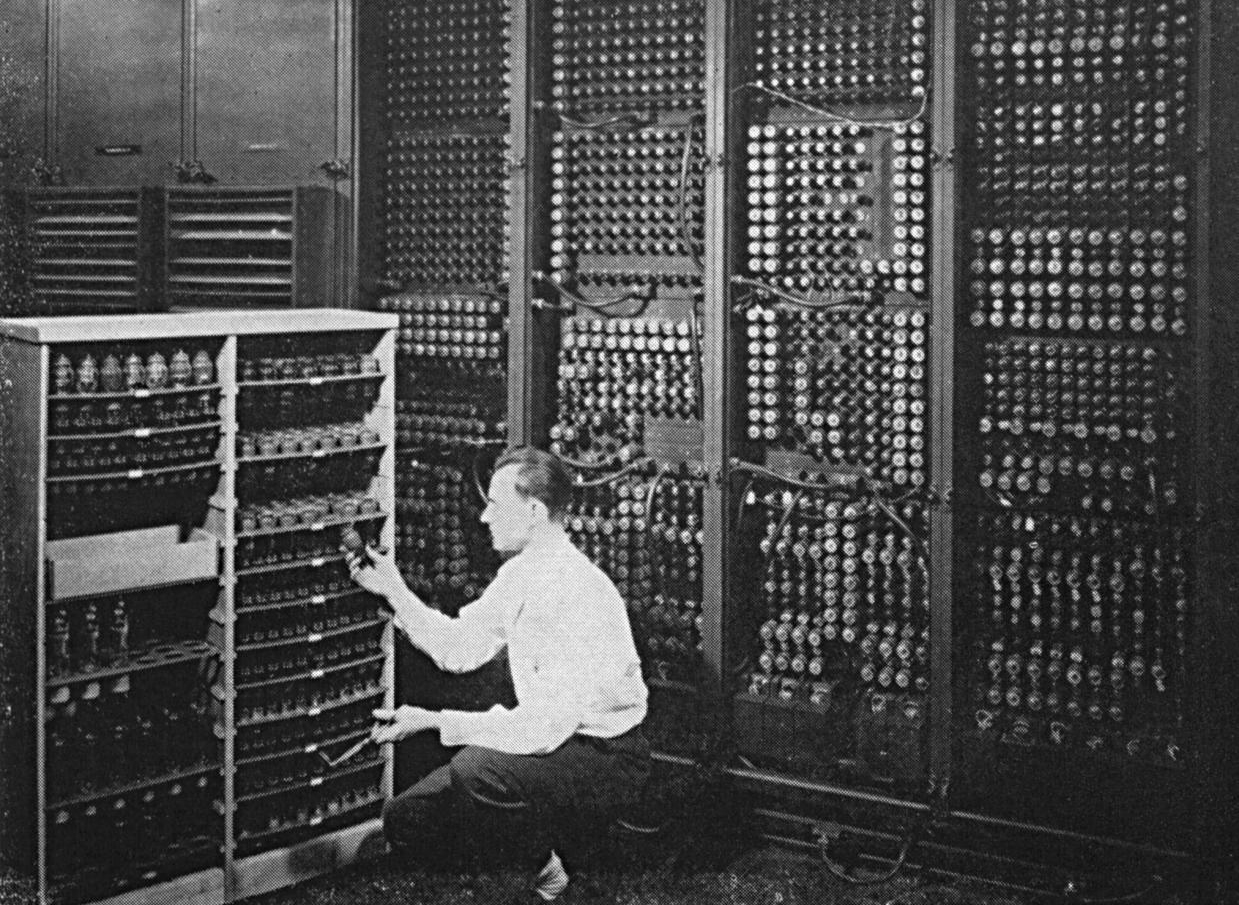
\includegraphics[width=0.7\linewidth]{eniacsvacuum}
	\caption[]{An ENIACS computer, which operated off of vacuum tubes\cite{ENIACS}.}
	\label{fig:eniacsvacuum}
\end{figure}


However, regular computers will soon reach the limit of how small these specialized transistors can get. Current CPU architecture is based off of 14 nanometer transistors. The next generation of transistors will reach 10 nanometers. \cite{Intel}
%https://www.intel.com/content/dam/www/public/us/en/documents/technology-briefs/bohr-14nm-idf-2014-brief.pdf
 Computer scientists predict that transistors will reach their physical limit size sometime in the mid 2020's. This limit is due to the fact that the transistors are approaching the size of atoms\cite{ARSTech}. Because of this asymptote, computers can no longer use an increase of transistor density for an speed boost. Another approach has to be derived. 
%https://arstechnica.com/gadgets/2016/07/itrs-roadmap-2021-moores-law/


\subsection{How Transistors Run A Computer}
How does a microscopic electronic component that can only be in 2 states operate a device that can perform billions of calculations per second? A transistor is a switch that can either be on or off to represent a 1 or a 0, respectively\footnote{Most computers use a 5V charge to signal an ON, and a 0V charge to signal an OFF \cite{Surrey}
	%http://www.ee.surrey.ac.uk/Projects/CAL/digital-logic/gatesfunc/
}. It will exist in exactly one of these states at any given time (in other words, a transistor cannot exist in a quasi-on state). One transistor by itself cannot do much. However, combining the transistors can result in extremely powerful calculations. Combining these transistors forms logical gates known as AND, OR,and NOT.  For an AND gate, the input is a pair of bits, and the output is a single bit. When both input bits are on, the output is is on, but otherwise, the output is off. Another type of gate is the OR gate. This has 2 inputs and 1 output. If either of the inputs is true, or both are true, the output is true. Only if both are false is the output false. 

For a NOT gate, the input is a single bit and the output is also a single bit. The output is simply the opposite of the input. 
%Source http://www.electronics-tutorials.ws/logic/logic_5.html

Combining these base transistors allows for other types of logic gates to be formed, including the XOR, NAND, NOR and XNOR gates.

 By placing a NOT gate on the output of an AND gate, a NAND gate is formed, which outputs the opposite of the AND gate. 

The XOR gate, also known as the eXclusive OR gate. Unlike the OR gate, the XOR gate will only show true if exactly 1 input is true. This is also known as the either/or gate.
\begin{figure}
	\centering
	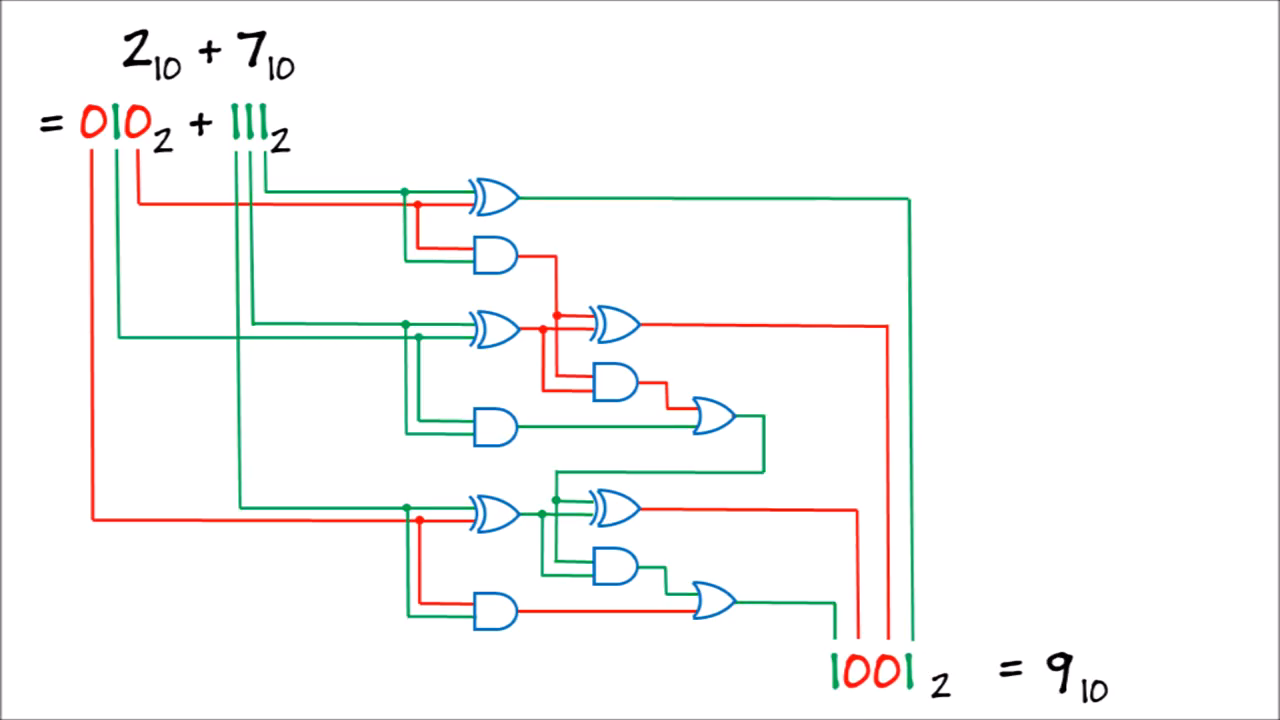
\includegraphics[width=0.7\linewidth]{adder}
	\caption{A sample setup using logic gates to add 2 numbers\cite{Essence}.}
	\label{ .}
\end{figure}


The combination of these logical gates results a boolean table known as a Truth Table\cite{Surrey}. This allows for very low level instructions, such as STORE, LOAD, ADD, or COMPARE. See Figure 2 above for a sample addition machine.

%https://youtu.be/F8U1d2Hqark?t=254
These instructions can be used to address the data stored in RAM. The language used for these instructions is called `assembly language' or `machine code'\footnote{This language is referred to as a low-level language, while more common languages like Python, FORTRAN, C/C++, and Java are referred to as high-level languages. This refers to the logical distance between the syntax of the language and the machine language, along with the amount of abstraction used in the language.}.

A quantum computer operates uses a slightly different principle. Instead of operating on a physical piece of hardware (the transistor) that produces a bit, quantum computers operate by observation of a photon that represents a qubit\footnote{Qubit is a juxtaposition of QUantum BIT}. A qubit is a special type of bit that can either represent a 1, a 0, or a superposition of a 1 and a 0. But how can something exist in both a 1 and a 0 at the same time? To understand this, one must first understand the principle behind Schr\"{o}dinger’s cat. 


The infamous Schr\"{o}dinger's cat experiment is performed as follows. Imagine a living cat inside a sealed bunker, with a sealed beaker of radioactive material, a Geiger counter attached to a hammer, and a small piece of radioactive material. As radioactive decay is a random process, the material has a 50\% chance of having one of its atoms decay in the next hour (which would set off the Geiger counter, smashing the hammer into the vial of gas and releasing it into the bunker, killing the cat). As long as the bunker is sealed and unobserved, the cat has a 50\% chance of being dead and a 50\% chance of being alive. When the bunker is opened, however, the cat must either be dead or alive. The instant before the bunker is opened, the cat exists in a quantum superposition of both dead and alive\cite{NatGeo}. 

Just like the cat, as long as the qubit is unobserved, it exists in a quantum superposition both a 1 and a 0. As soon as the qubit is observed, it ``snaps'' to either a 1 or a 0. Another way of thinking about this is like a coin that is flipped and is  spinning in midair. At any point in the air, it is practically impossible to figure out if the orientation of the coin is heads or tails. However, smashing a fist down on top of the coin will force it to go to either a heads or a tails orientation. But how does this help a quantum computer work faster than a regular computer?


% needed in second column of first page if using \IEEEpubid
%\IEEEpubidadjcol

\subsection{How a Quantum Computer can solve NP-type problems}

The operations of a computer can be compared to an office worker sitting at their desk. The storage (hard drive) is comparable to a file cabinet for long term storage. The Random Access Memory (RAM, also known as memory) is comparable to the top of the desk, where papers can be placed when they are being worked on. Finally, the CPU is comparable to the person sitting at the desk, actually performing the tasks. The person can only work on something on the top of their desk, as trying to read a piece of paper sitting in a file cabinet would be awkward and slow\footnote{Interestingly enough, trying to work on a paper while the paper is still in the file cabinet can be compared to a pagefile, where the CPU pulls data directly from storage.}. Therefore, the person pulls an item out of their file cabinet and places it on their desk. The desk can only hold so many papers, so when the desk runs out of room, some papers have to be put back into the file storage. 




Similiarly to the desk analogy, a CPU instructs the hard drive to load certain pieces of information from the hard drive into the RAM. When the computer runs out of free memory, the CPU removes information from the RAM that isn't being used. Unlike the desk analogy, however, the CPU does not directly operate from the RAM. Instead, the CPU loads a small bit of information from the RAM into the register of the CPU. The register is a very small amount of extremely fast storage directly tied to the CPU. For example, an Intel i7 CPU has 64 bit, 80 bit, and 120 bit registers\footnote{Compare these register sizes to the RAM in an average desktop, which is measured in gigabytes.}. Once in the register, the bits go through the transistors discussed earlier, where the logical gates perform instructions based on the data going through them\cite{THPHYS}\cite{Explain}.


%Source
%http://www.explainthatstuff.com/quantum-computing.html

%SOURCE http://www.thphys.nuim.ie/staff/joost/TQM/QvC.html

The bits in a classical computer have a value of 1 or 0. This is relatively efficient, but storing an N-bit number requires N bits. In other words, storing a 64 bit value takes 64 bits, and storing a 256 bit value takes 256 bits. The transistors in the CPU only recognize the 2 states, and operate serially (in series) on each bit. 

A quantum computer, on the other hand, uses bits that exist in a state that is either a $|1\}$, a $|0\}$, or a superposition that can be represented with the expression $a|1\} + b|0\}$. The state of the bit can be expressed using complex vector addition, varying the values of $a$ and $b$. However, due to a quantum theory known as quantum entanglement, the state of 1 qubit affects the other qubits in the system. Two particles can be entangled even if they are separated by physical space. Due to the entanglement, the qubits allow for exponentially growing identification of bits. N qubits can represent $2^N$ classical bits. A very critical point about this: quantum computers do not measure the values of the individial qubits. Instead, they measure the ``correlations'', or interactions, between the qubits. Just like Schr\"{o}dinger's cat, as soon as the qubits themselves are observed, the system changes from its original state. The cutting link to success came when two computers scientists, David Deutsch and Richard Jozsa, determined an algorithm that allowed for a computer to deduce what the original state of the qubits was most likely to have been before observation. Think of it like a house of cards that cannot be observed without them falling into a pile. The Jozsa-Deutsch algorithm allows for a computer to determine the most likely original state of the cards. Although the exact original state cannot be determined in a single computational run, by running multiple computations, the computer can deduce what the most likely original state of the qubits was, which will result in the solution to the problem\cite{NIST}.

%Algorithm link https://www.quantiki.org/wiki/deutsch-jozsa-algorithm

This ability is what makes a quantum computer so powerful. Instead of operating serially on a stream of bits, the computer can operate in parallel, on multiple bits simultaneously. This capability, combined with the right algorithm, will be able to solve a NP problem in polynomial time. 

% An example of a floating figure using the graphicx package.
% Note that \label must occur AFTER (or within) \caption.
% For figures, \caption should occur after the \includegraphics.
% Note that IEEEtran v1.7 and later has special internal code that
% is designed to preserve the operation of \label within \caption
% even when the captionsoff option is in effect. However, because
% of issues like this, it may be the safest practice to put all your
% \label just after \caption rather than within \caption{}.
%
% Reminder: the "draftcls" or "draftclsnofoot", not "draft", class
% option should be used if it is desired that the figures are to be
% displayed while in draft mode.
%
%\begin{figure}[!t]
%\centering
%\includegraphics[width=2.5in]{myfigure}
% where an .eps filename suffix will be assumed under latex, 
% and a .pdf suffix will be assumed for pdflatex; or what has been declared
% via \DeclareGraphicsExtensions.
%\caption{Simulation results for the network.}
%\label{fig_sim}
%\end{figure}

% Note that the IEEE typically puts floats only at the top, even when this
% results in a large percentage of a column being occupied by floats.
% However, the Computer Society has been known to put floats at the bottom.


% An example of a double column floating figure using two subfigures.
% (The subfig.sty package must be loaded for this to work.)
% The subfigure \label commands are set within each subfloat command,
% and the \label for the overall figure must come after \caption.
% \hfil is used as a separator to get equal spacing.
% Watch out that the combined width of all the subfigures on a 
% line do not exceed the text width or a line break will occur.
%
%\begin{figure*}[!t]
%\centering
%\subfloat[Case I]{\includegraphics[width=2.5in]{box}%
%\label{fig_first_case}}
%\hfil
%\subfloat[Case II]{\includegraphics[width=2.5in]{box}%
%\label{fig_second_case}}
%\caption{Simulation results for the network.}
%\label{fig_sim}
%\end{figure*}
%
% Note that often IEEE papers with subfigures do not employ subfigure
% captions (using the optional argument to \subfloat[]), but instead will
% reference/describe all of them (a), (b), etc., within the main caption.
% Be aware that for subfig.sty to generate the (a), (b), etc., subfigure
% labels, the optional argument to \subfloat must be present. If a
% subcaption is not desired, just leave its contents blank,
% e.g., \subfloat[].


% An example of a floating table. Note that, for IEEE style tables, the
% \caption command should come BEFORE the table and, given that table
% captions serve much like titles, are usually capitalized except for words
% such as a, an, and, as, at, but, by, for, in, nor, of, on, or, the, to
% and up, which are usually not capitalized unless they are the first or
% last word of the caption. Table text will default to \footnotesize as
% the IEEE normally uses this smaller font for tables.
% The \label must come after \caption as always.
%
%\begin{table}[!t]
%% increase table row spacing, adjust to taste
%\renewcommand{\arraystretch}{1.3}
% if using array.sty, it might be a good idea to tweak the value of
% \extrarowheight as needed to properly center the text within the cells
%\caption{An Example of a Table}
%\label{table_example}
%\centering
%% Some packages, such as MDW tools, offer better commands for making tables
%% than the plain LaTeX2e tabular which is used here.
%\begin{tabular}{|c||c|}
%\hline
%One & Two\\
%\hline
%Three & Four\\
%\hline
%\end{tabular}
%\end{table}


% Note that the IEEE does not put floats in the very first column
% - or typically anywhere on the first page for that matter. Also,
% in-text middle ("here") positioning is typically not used, but it
% is allowed and encouraged for Computer Society conferences (but
% not Computer Society journals). Most IEEE journals/conferences use
% top floats exclusively. 
% Note that, LaTeX2e, unlike IEEE journals/conferences, places
% footnotes above bottom floats. This can be corrected via the
% \fnbelowfloat command of the stfloats package.




\section{Effects of Quantum Computing}
\IEEEPARstart{W}{hat} effects will the rise of a general purpose quantum computer have on real life applications? Several benefits are readily apparent, including military interception of foreign messages, optimization of route generation, and advancement of artificial intelligence. However, several drawbacks exist, the two most critical being encryption techniques and blockchain. 
\subsection{Cryptography}
The United States Military expresses a large amount of interest in quantum computing, primarily for its use in cryptanalysis, or code-breaking. Cracking a code is defined as an NP problem, as the difficulty of the problem increases exponentially as the length of the message grows. Because quantum computers can analyze large numbers of bits simultaneously, they are excellent for problems that require brute force calculations. This allows for the breaking of coded messages from enemy intelligence, ultimately allowing for an advantage over the enemy to successfully complete a mission while saving lives. 

\subsection{Route Generation}
Another use of quantum computing arises in finding the shortest route between a set of points. Imagine a door-to-door salesman, with a set of houses he has to visit. To find the most efficient route to visit all of these houses requires a brute force approach. Guessing a random route, as well as measuring the length of that route are both extremely easy problems, classified as P difficulty. However, determining the shortest route is considered an NP problem\footnote{See Appendix C }.
%http://mathworld.wolfram.com/TravelingSalesmanProblem.html
In math terms, this problem is attempting to find the most efficient Hamiltonian Cycle to take through a set of N nodes. In more simplified terms, this is finding the shortest route between a set of random points. One practical application of this is route generation for logistics management companies. 

Logistics companies such as the United Postal Service (UPS) deliver millions of packages every day, with the route changing daily. But finding the shortest path is not the only issue. Certain packages must be delivered before others, due to priority shipping methods (the customer who paid for priority overnight express will get his package delivered before the customer who paid for the base shipping rate). The current algorithms use a heuristic approach, approximating the best route and using "rules of thumb", resulting in sub-optimal routes. Again, the only way to find the best route currently is with brute force, which is impossible with classical computing. In fact, the number of possible routes for a single UPS truck to take daily exceeds the the number of nanoseconds that the Earth has existed\cite{Fast}. With quantum computing, this calculation would be able to be solved in polynomial time, allowing UPS to find optimal routes for all of its trucks. This would allow for both time and money to be saved. Furthermore, because the trucks are traveling less on the road, they are emitting less pollution. 


 
 \subsection{Artificial Intelligence}
One highly important section of the field of quantum computing is its application in the field of artificial intelligence. According to IBM, one such application is "Making facets of artificial intelligence such as machine learning much more powerful when data sets are very large, such as in searching images or video."\cite{IBM} Machine learning (such as IBM's Watson) relies on searching a vast database of information to calculate results. As the size of the database increases, the length of time to search for the required information also increases. Through the use of quantum computing, these database searches can be completed on orders of magnitude faster than would be possible with standard computing methods\cite{IBM}. 

The initial drawbacks for most usage would be the cost of the hardware, as well as developing the complex algorithms that can properly run on quantum-based hardware. However, as with most all first-generation hardware, the initial cost is astronomically high. If quantum computers follow anything like the path of classical computers' development, the price will soon drop, allowing companies to use quantum algorithms in the use of artificial intelligence, turning a high-cost item into a cost-effective alternative. 
 %http://www.research.ibm.com/ibm-q/learn/quantum-computing-applications/

The many benefits of quantum computing seem to point towards a positive outlook. However, as with any technology, there will always be drawbacks. 
 

\subsection{RSA Encryption}

As a shopper enters their credit card details for an online store website, the shopper is assured that their credit card details and other personal data are protected if the green lock icon is present in their browser. The only reason this lock icon has any significant value is thanks to two major points: 

1) Prime factorization is classified as an NP problem

2) the difficulty of cracking this encryption (known as RSA encryption) is extremely difficult and time consuming using current computation methods. 

In 1978, three computer scientists, Ron Rivest, Adi Shamir and Leonard Adleman, publicly released an encryption algorithm titled after their names, RSA \cite{RSA}. The basis of this asymmetric encryption technique\footnote{Please note that this is a highly simplified explanation of the encryption algorithm. To describe this in full detail would take far more in-depth explanations and mathematics than would be appropriate for this paper.} is two secret prime numbers (known as private keys) multiplied together to form a public key. To decrypt the message, the two original numbers must be known. Finding these original two numbers is only possible through repetitive brute force calculations\footnote{Although  some algorithms exist to reduce the work slightly using methods to eliminate groups of guesses, it is still a polynomial reduction on an exponential growth, which means the reduction is almost unnoticeable.}. For an idea of the size of these numbers, the public key length for most banking systems nowadays is over six hundred digits long\footnote{A 617 digit long public key is the key length for 2048 bit encryption.}\cite{Numberphile}. To complete these calculations with current  methods and computing technologies  would require somewhere on the order of 6.4 quadrillion years to try all possible combinations. 

However, with quantum computing's parallel computation techniques, multiple factors can be tried simultaneously, cutting the time to crack an encryption drastically. This is not just a science fiction threat, though. Previously, a variant of RSA cryptography known as elliptic curve cryptography\footnote{Elliptic curve cryptography is an encryption method similar to RSA that uses discrete logarithms of elliptic curves to choose the private keys. However, it still operates off of the same principle, with a private key and a public key related to each other through irreversable complex mathematical algorithms.} was approved by the National Security Administration (NSA) as the minimum for encryption standards of private data. In August of 2017, the NSA released a statement about the threat from quantum computing:

"For those vendors and partners that have already transitioned to Suite B [elliptic curve cryptography], we recognize that this took a great deal of effort on your part, and we thank you for your efforts. … Unfortunately, the growth of elliptic curve use has bumped up against the fact of continued progress in the research on quantum computing, which has made it clear that elliptic curve cryptography is not the long term solution many once hoped it would be. Thus, we have been obligated to update our strategy."\cite{Information}

In other words, even the NSA is concerned with the rise of quantum computing. Furthermore, any data that is currently stored with non-post-quantum cryptography methods  will be subject to cracking within the next few decades at most. 

Many major organizations, such as Internet Service Providers (ISPs) and the NSA store user data in an encrypted (and currently secure) manner. The sole reason this data is secure is because of the reliance in standard encryption methods. If a quantum computer is developed by a malicious source (foreign or domestic), everyone's so-called "private" information is at imminent risk of being decoded and stolen. 

\subsection{Blockchain and Cryptocurrencies}
Yet another aspect of technology that would be affected with quantum computing is the use of blockchain for cryptocurrencies. In technical terms, blockchain is a public peer-to-peer ledger to account for and validate transactions of a decentralized cryptocurrency, such as Bitcoin, Ethereum, and Monero. 

The most commonly used cryptocurrency is Bitcoin; however, almost all cryptocurrencies operate off of the same general principle\cite{Bitcoin}. 

When Alice wants to transfer some amount of Bitcoin to Bob, the transaction information is stored in the ledger, which is a public record of all of the transactions that have occurred. The records include Alice and Bob's "wallet" ID's, as well as the the amount transferred. Groups of transactions are collected into a block. These blocks are chained together (hence the name), and then a "pointer" refers each block to the previous block. 

Where do these blocks come from? They originate  from the maintainers of the ledger. Unlike a bank, where a central authority confirms transactions, cryptocurrencies are decentralized. The maintainers of the ledger are known as `miners', which are computers with special hardware optimized for solving large amounts of math problems\cite{Aggarwal}. When Alice sends Bob a certain value of Bitcoin, this value is recorded in the public ledger. Other miners on the network run this information through a hashing algorithm known as SHA256. For example, if Alice sends Bob 2 bitcoin, a value would be added to the ledger saying something like ALICE-2 BOB+2. At this point, anyone could theoretically change the value of 2 Bitcoin to any value desired\footnote{Note that the actual value added to the ledger is far more complicated. This is just a psuedocode explanation of the general process.}. Therefore, the value added to the ledger is hashed. Hashing is an algorithm that gives a standard size output for any size input, where even a slight change in the input results in a drastically different ouput. For reasons beyond the scope of this paper, miners must plug in random values into the hashing algorithm to verify the output. Once a majority of miners agree on the output, that value is set in stone as the correct value. 

The security of cryptocurrencies relies on the assumption that no individual will ever control more than 50\% of the network\cite{Futurism}. Once this happens, the majority control can be used maliciously in various ways, the most egregious being that an alternate history of transactions in the ledger could be passed off as truthful. This means that malicious parties could theoretically manipulate an entire currencies value, as well as steal currency from other users. 

%Bitcoin threat paper
%https://arxiv.org/pdf/1710.10377.pdf

%Source of bitcoin
%https://bitcoin.org/en/how-it-works

%Source for BCN threat
%futurism.com/bitcoins-security-quantum-computers/

%Explanatnio for bitcoin
%https://www.youtube.com/watch?v=t5JGQXCTe3c



\section{Conclusion}
\IEEEPARstart{O}{nce a reliable} general purpose quantum computer is available, the face of mathematics will be changed forever. Math and science problems that would not have been possible before will now be able to be accomplished in mere seconds. Some benefits include the use of quantum computing for cryptanalysis to aid military intelligence, optimal route generation for logistics companies, and optimization of data retrieval for artificial intelligence. 

But as with all new technology, there will always be drawbacks. These include the misuse of quantum computing to both crack commonly used encryption methods and destroy the cryptocurrency economy.

As an unknown author once said, "Computers are incredibly fast, powerful, and stupid. Humans are incredibly slow, innacurate, and brilliant. Together, they are powerful beyond imagination."

% if have a single appendix:
%\appendix[Proof of the Zonklar Equations]
% or
%\appendix  % for no appendix heading
% do not use \section anymore after \appendix, only \section*
% is possibly needed

% use appendices with more than one appendix
% then use \section to start each appendix
% you must declare a \section before using any
% \subsection or using \label (\appendices by itself
% starts a section numbered zero.)
%


\appendices
\section{Sample Code for Largest Element}
Assume the list of numbers is stored in a list named $num\_list$. The following is written in Python. Note how there is only 1 FOR loop.
\begin{lstlisting}
greatest_element = num_list[0]
for element in num_list:
	if element>greatest_element:
		element = greatest_element
return element

\end{lstlisting}

% you can choose not to have a title for an appendix
% if you want by leaving the argument blank
\section{Proof of iteration count for sacks}
Start with a test case, then prove for a general solution. 
Let the number of sacks in the initial collection be $4$. 

To figure out the total possible number of sacks, use a case by case scenario. Every final count of sacks will either contain 1, 2, 3, or 4 sacks. 
\begin{itemize}
	\item \textbf{Case 1}, picking 4 sacks. \\
	There are 4 possible choices for the first sack, 3 possible for the second, 2 for the third, and 1 for the fourth. Mathematically represented, there are  $\Perm{4}{4} = 4! = 4\cdot3\cdot2\cdot1$ possible combinations. However, as the order the sacks are picked in does not matter (picking sacks 1,2,3, and 4 is the same as picking sacks 3,2,4, and 1), divide by $4!$. The mathematical represenatation of this compensation is $\Comb{4}{4}$. $$\frac{4!}{4!} = 1$$ This makes sense, because there's only 1 way to pick a collection of all 4 sacks. 
	\item \textbf{Case 2}, picking 3 sacks.\\
	With the same logic as the previous case, there are  $\Perm{4}{3} = 4\cdot3\cdot2$  possible unordered combinations. However, each choice of 3 sacks can be arranged in $3!$ ways, so therefore divide the total number of collections $(4!)$ by the number of arrangements of each $(3!)$. $$\frac{4!}{3!} = \frac{24}{6} = 4$$
	\item \textbf{Case 3}, picking 2 sacks.\\
	\[\Comb{4}{2} = \frac{\Perm{4}{2}}{2!} = 6\]
	\item \textbf{Case 4}, picking 1 sack.\\
	\[\Comb{4}{1} = \frac{\Perm{4}{1}}{1!} = 4\]
	Adding each of these together results in $1+4+6+4 = 15$. 
	
	The number of possible combinations for each case is not a random number. These numbers actually come from the Binomial Coefficients of Pascal's Triangle. 
	\begin{tabular}{rccccccccc}
		$n=0$:&    &    &    &    &  1
		\\\noalign{\smallskip\smallskip}
		$n=1$:&    &    &    &  1 &    &  1\\\noalign{\smallskip\smallskip}
		$n=2$:&    &    &  1 &    &  2 &    &  1\\\noalign{\smallskip\smallskip}
		$n=3$:&    &  1 &    &  3 &    &  3 &    &  1\\\noalign{\smallskip\smallskip}
		$n=4$:&  1 &    &  4 &    &  6 &    &  4 &    &  1\\\noalign{\smallskip\smallskip}
	\end{tabular}
	
	The row $n=4$ has the same values as each of the cases discussed above. (The only number that does not show is the first 1, as this represents the number of ways to pick zero elements from the list of initial sacks. As this is not a valid solution to the problem, it is ignored.)
\end{itemize}

\section{Traveling Salesman NP Proof}
A simple explanation behind this statement: To find the shortest route between a set of nodes $N_1,N_2,\cdots N_Q$ of size Q, start at any node $N_1$. At this point, $Q$ guesses have been checked. Now, there are $Q-1$ points left to try. After another point $N_2$ has been selected, $Q(Q-1)$ guesses have been attempted. After another point, the number of guesses goes to $Q(Q-1)(Q-2)$. This is increasing at a rate of $Q!$, which is a non-polynomial growth. 


\section{Self-Assessment}
This paper definitely challenged my knowledge of computing techniques. The strongest part of my paper is the explanations of complex ideas, putting them into terms that an average person without a strong knowledge of computing would understand. The weakest part of my paper is the explanation of how a quantum computer exactly works. The reason for this is because my knowledge of quantum computing is still very limited. 


% use section* for acknowledgment
\ifCLASSOPTIONcompsoc
  % The Computer Society usually uses the plural form
  \section*{Acknowledgments}
\else
  % regular IEEE prefers the singular form
  \section*{Acknowledgment}
\fi


The author would like to thank Dr Gaines Hubbel, for his amazing EH105 class, as well as the author's family and friends for proofreading. The author would also like to give a shoutout to Carrie, for her late night sanity checks. Furthermore, the author would like to thank Dunkin Donuts, Reddit ELI5, StackOverflow, and Wikipedia, without which he would have no clue what he was talking about.


% Can use something like this to put references on a page
% by themselves when using endfloat and the captionsoff option.
\ifCLASSOPTIONcaptionsoff
  \newpage
\fi



% trigger a \newpage just before the given reference
% number - used to balance the columns on the last page
% adjust value as needed - may need to be readjusted if
% the document is modified later
% \IEEEtriggeratref{8}
% The "triggered" command can be changed if desired:
%\IEEEtriggercmd{\enlargethispage{-5in}}

% references section

% can use a bibliography generated by BibTeX as a .bbl file
% BibTeX documentation can be easily obtained at:
% http://mirror.ctan.org/biblio/bibtex/contrib/doc/
% The IEEEtran BibTeX style support page is at:
% http://www.michaelshell.org/tex/ieeetran/bibtex/
%\bibliographystyle{IEEEtran}
% argument is your BibTeX string definitions and bibliography database(s)
%\bibliography{IEEEabrv,../bib/paper}
%
% <OR> manually copy in the resultant .bbl file
% set second argument of \begin to the number of references

\begin{thebibliography}{1}
	\bibitem{NSA}
	Nsa.gov. (n.d.). NSA Declassified Documents. [online] Available at: www.nsa.gov/news-features/declassified-documents/nash-letters/assets/files/nash\_letters1.pdf [Accessed 25 Nov. 2017].

	\bibitem{Britannica}
	"Theorem of Prime Factorization", Encyclopedia Britannica, 2017. [Online]. Available: https://www.britannica.com/topic/fundamental-theorem-of-arithmetic. [Accessed: 27- Nov- 2017].
	
	\bibitem{URI}
	"History of Computers", Homepage.cs.uri.edu, 2017. [Online]. Available: homepage.cs.uri.edu/faculty/wolfe/book/Readings/Reading03.htm. [Accessed: 25- Nov- 2017].
	
	\bibitem{Tom's}
	"Computer History 101: The Development Of The PC", www.tomshardware.com, 2011. [Online]. Available: www.tomshardware.com/reviews/upgrade-repair-pc,3000-2.html, [Accessed: 25-Nov-2017]	
	
	\bibitem{Moore}
	S. Shankland, "Moore's Law: The rule that really matters in tech", CNET, 2017. [Online]. Available: www.cnet.com/news/moores-law-the-rule-that-really-matters-in-tech/. [Accessed: 25- Nov- 2017].	
	

	
	\bibitem{Intel}
	"14nm Process Technology: Opening New Horizons", Intel Developer Forum, San Francisco, CA, 2017.
	
	\bibitem{ENIACS}
	Computer History Museum, ENIACS Tube Change. 2017.


	\bibitem{ARSTech}
	S. Anthony, "Transistors will stop shrinking in 2021, but Moore’s law will live on", ARSTechnica, 2017. [Online]. Available: arstechnica.com/gadgets/2016/07/itrs-roadmap-2021-moores-law/. [Accessed: 25- Nov- 2017].

	\bibitem{Surrey}
	W. Sangosanya, "Basic Logic Gates", Ee.surrey.ac.uk, 2017. [Online]. Available: www.ee.surrey.ac.uk/Projects/CAL/digital-logic/gatesfunc/. [Accessed: 25- Nov- 2017].
	
	\bibitem{Essence}
	Frame of Essence, Building the Bits and Qubits. 2017.


	\bibitem{NatGeo}
	M. Kramer, "The Physics Behind Schrödinger's Cat Paradox", News.nationalgeographic.com, 2017. [Online]. Available: news.nationalgeographic.com/news/2013/08/130812-physics-schrodinger-erwin-google-doodle-cat-paradox-science/. [Accessed: 25- Nov- 2017].	

	\bibitem{THPHYS}
	"Quantum vs Classical Computation", Thphys.nuim.ie, 2017. [Online]. Available: http://www.thphys.nuim.ie/staff/joost/TQM/QvC.html. [Accessed: 26- Nov- 2017].
	
	\bibitem{Explain}
	Woodford, Chris. (2012/2017) Quantum computing. Retrieved from http://www.explainthatstuff.com/quantum-computing.html. [Accessed (26- Nov- 2017)] 	
	

	\bibitem{NIST}
	Paul E. Black, "Deutsch-Jozsa algorithm", in Dictionary of Algorithms and Data Structures [online], Vreda Pieterse and Paul E. Black, eds. 17 December 2004. (accessed 25-Nov-2017) Available from: www.nist.gov/dads/HTML/deutschJozsaAlgo.html	
	
	\bibitem{Fast}
	D. Zax, "Brown Down: UPS Drivers Vs. The UPS Algorithm", Fast Company, 2017. [Online]. Available: www.fastcompany.com/3004319/brown-down-ups-drivers-vs-ups-algorithm. [Accessed: 26- Nov- 2017].
	

	\bibitem{IBM}
	"Quantum computing applications - IBM Q - US", Research.ibm.com, 2017. [Online]. Available: www.research.ibm.com/ibm-q/learn/quantum-computing-applications/. [Accessed: 25- Nov- 2017].


	
	\bibitem{RSA}
	G. Simmons, "Rivest-Shamir-Adleman encryption", Encyclopedia Britannica, 2017. [Online]. Available: www.britannica.com/topic/RSA-encryption. [Accessed: 25- Nov- 2017].

	
	\bibitem{Numberphile}
	Encryption and HUGE numbers. Youtube: Numberphile, 2012

	\bibitem{Information}
	"Information Assurance--Suite B Cryptography", Nsa.gov,2017. [Online]. Available: www.nsa.gov/ia/programs/suiteb\_cryptography/index.shtml. [Accessed: 26- Nov- 2017].

	\bibitem{Bitcoin}
	"How does Bitcoin work? - Bitcoin", Bitcoin.org, 2017. [Online]. Available: https://bitcoin.org/en/how-it-works. [Accessed: 26- Nov- 2017].
	
	\bibitem{Aggarwal}
	D. Aggarwal, G. Brennen, T. Lee, M. Santha and M. Tomamichel, "Quantum attacks on Bitcoin, and how to protect against them", Arxiv.org, 2017. [Online]. Available: https://arxiv.org/abs/1710.10377. [Accessed: 26- Nov- 2017].
	
		
	\bibitem{Futurism}
	D. Galeon, "Experts: "Quantum computers will break Bitcoin security within 10 years"", Futurism, 2017. [Online]. Available: https://futurism.com/bitcoins-security-quantum-computers/. [Accessed: 26- Nov- 2017].


%%%%%%%%%%%%%%%%%%%%%%%%%%%%
%Unordered below here

	
	
	


	
	

	
%	\bibitem{Turing}
%	A. Hodges, "Alan Turing", Plato.stanford.edu, 2017. [Online]. Available: plato.stanford.edu/entries/turing/. [Accessed: 25- Nov- 2017].
	





	
		

	

\end{thebibliography}



% that's all folks
\end{document}
